% Document Type: LaTeX
% Master File: thesis.tex
\documentclass[12pt,a4paper]{report}
\usepackage{fcthesis}         %estilo da tese (``uptese'' --> portugues)
% \usepackage[ingles]{babel}
\usepackage[utf8]{inputenc}
%\usepackage{epsf}             %incluir figuras encapsulated postscript
%\usepackage{amstex}
%\pagestyle{myheadings}

%%%%%%%%%%%%%%%%%%%%%%%%%%%%%%%%%%%%%%%%%%%%%%%%%%%%%%%%%%%%%%%%%
\usepackage{tikz}
\usepackage{listings}
\usepackage{color}

%\usepackage{graphicx}
%\usepackage{graphics}

\graphicspath{ {./images/} }

\usetikzlibrary{shapes,shapes.geometric,arrows,fit,calc,positioning,automata,decorations.pathmorphing}

\definecolor{codegreen}{rgb}{0,0.6,0}
\definecolor{codegray}{rgb}{0.5,0.5,0.5}
\definecolor{codepurple}{rgb}{0.58,0,0.82}
\definecolor{backcolour}{rgb}{0.95,0.95,0.92}

\lstdefinestyle{mystyle}{
    backgroundcolor=\color{backcolour},
    commentstyle=\color{codegreen},
    keywordstyle=\color{magenta},
    numberstyle=\tiny\color{codegray},
    stringstyle=\color{codepurple},
    basicstyle=\footnotesize,
    breakatwhitespace=false,
    breaklines=true,
    captionpos=b,
    keepspaces=true,
    numbers=left,
    numbersep=5pt,
    showspaces=false,
    showstringspaces=false,
    showtabs=false,
    tabsize=2
}
\lstset{style=mystyle}

\usepackage{amsthm}
\usepackage{subcaption}

\theoremstyle{definition}
\newtheorem{definition}{Definition}
\newtheorem{theorem}{Theorem}
\newtheorem{corollary}{Corollary}
\newtheorem{lemma}[theorem]{Lemma}

\renewcommand\lstlistingname{Algorithm}
\renewcommand\lstlistlistingname{Algorithms}

%%%%%%%%%%%%%%%%%%%%%%%%%%%%%%%%%%%%%%%%%%%%%%%%%%%%%%%%%%%%%%%%%

\includeonly{abs,decl,pref,acks,ch1,ch2,ch3,ch4,app1}

\begin{document}

\title{Degree of Ambiguity}

\submitionplace{Relatório de Projeto}

\author{Afonso das Neves Fernandes}
\department{Departamento de Ci\^encia de Computadores \\ Faculdade de
Ci\^encias da Universidade do Porto}

\submitdate{Junho de 2019}

\supervisor{Nelma Resende Araújo Moreira e Rogério Ventura Lages dos Santos Reis}
% \cosupervisor{Nome Completo (se aplicável, retirar caso contrário)}

\beforepreface
% \dedicationpage{(Dedicat\'oria opcional...)}
% \include{acks}
% \include{pref}
% \include{abs}
\afterpreface

% end of thesis preambule
\lstlistoflistings
\chapter{Introduction}
One important subject in computer science is theory of finite automata because automata are a robust model of computation that has widespread applications from compilers to bioinformatics, image recognition and computer networks.

One of such applications is in pattern matching and in particular regular expression pattern matching. For manipulation, expressions are usually converted into non-deterministic finite automata. One of the difficulties is the ambiguity of the automata because there may exist several possible matches and thus several syntactic trees. To prevent these problems, normally, greedy strategies are implemented to select one \cite{BorsottiBCM15}.

In this report, we will study the ambiguity of non-deterministic finite automata. In particular we will use the library of FAdo \cite{BRODA201994} to implement the criteria for ambiguity classification and run experiments to study the distribution of the classes of ambiguity.

We start by defining ambiguity of an automaton and the classes of ambiguity. Then we present the criteria to classify the ambiguity and their implementations.

Finally, we will present the experiments done in order to study the distribution of the classes of ambiguity and discuss the results.

\section{Definitions and Notations}
In this section we present some definitions used in this report. In particular the definition of an NFA and a DFA, and the definition of a path.

% \begin{definition}
% An language is a set of words over an alphabet $\Sigma$.
% \end{definition}

Given a finite set of symbols $\Sigma$, called an alphabet, and a word as a finite sequence of elements of $\Sigma$, we define a language to be a set of words over an alphabet and $\Sigma^*$ to be the language of all words that can be formed using symbols of $\Sigma$.

Throughout this report, we use some simple regular expressions with the following operations: concatenation, $+$ as disjunction and $*$ as the Kleene star.

\begin{definition}
A non-deterministic finite automaton (NFA) M is defined as a $5$-tuple ($Q$,$\Sigma$,$\delta$,$I$,$F$) where $Q$ is the set of states, $\Sigma$ the set of input symbols, $\delta \subseteq Q \times \Sigma \times Q$ the finite set of transitions and $I$,$F$ are the set of initial and final states, respectively.
\end{definition}

The size of an NFA is defined as $|Q|+|\delta|$, the number of states plus the number of transitions.

% $\delta$ is the partial transition function defined as $Q \times \Sigma \mapsto 2^Q$

\begin{definition}
A deterministic finite automaton (DFA) is an NFA where for each state $s$ and symbol $x$ there is at most one pair ($s$,$x$,$s'$) in $\delta$, with $s'$ in $Q$.
\end{definition}

\begin{definition}
A path $\pi$ on an NFA is a sequence of states, bigger than one, such that between two consecutive states of $\pi$ there is at least one transition. We denote by $i[\pi]$ and by $f[\pi]$ the origin state and destination state of $\pi$. If $i[\pi] \in I$ and $f[\pi] \in F$ the path $\pi$ is an accepting path. A path $\pi$ is labeled by a set of words, each one resulting from the concatenation of symbols of the transitions between consecutive states of $\pi$ ($l[\pi]$). A path $\pi$ spells a word $w \in \Sigma^*$ if $w \in l[\pi]$.
A path accepts a word if it is an accepting path and if the path spells the word.
\end{definition}

% We define a path of an automata because it allows to define ambiguity of an automata in the next chapter.

\begin{figure}[ht]
\begin{subfigure}{.5\textwidth}
  \centering
  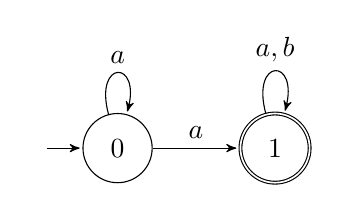
\begin{tikzpicture}[>=stealth', shorten >=1pt, auto,
    node distance=2cm,initial text={}]
    \node [state, initial]                           (A) {$0$};
    \node [state, accepting] [right of=A]            (B) {$1$};
    \path[->] (A) edge                          node {$a$} (B)
                  edge [loop above]             node {$a$} ()
              (B) edge [loop above]             node {$a,b$} ();
  \end{tikzpicture}
  \caption{NFA}
  \label{fig:nfa}
\end{subfigure}
\begin{subfigure}{.5\textwidth}
  \centering
  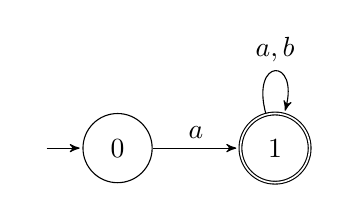
\begin{tikzpicture}[>=stealth', shorten >=1pt, auto,
    node distance=2cm,initial text={}]
    \node [state, initial]                           (A) {$0$};
    \node [state, accepting] [right of=A]            (B) {$1$};
    \path[->] (A) edge                          node {$a$} (B)
                  % edge [loop above]             node {$a$} ()
              (B) edge [loop above]             node {$a,b$} ();
  \end{tikzpicture}
  \caption{DFA}
  \label{fig:dfa}
\end{subfigure}
\caption{Example of an NFA and a DFA}
\label{fig:automaton_example}
\end{figure}

In figure \ref{fig:automaton_example} are shown two automata diagrams. The circles represent states and the arrows represent transitions.

In Figure \ref{fig:nfa} we have the following paths:
\begin{itemize}
  \item $\pi_1 = 0,0,1$
  \item $\pi_2 = 0,1,1$
\end{itemize}

The path $\pi_1$ is an accepting path and is labeled only by the word $aa$. On the other hand, the path $\pi_2$ is not an accepting path and is labeled by $\{aa,ab\}$

\begin{definition}
The language of an NFA $M$, $L(M)$, is the union of $l[\pi]$ for all accepting paths $\pi$ on $M$.
\end{definition}

All languages that can be represented by finite automata are called regular languages. If two automata accept the same language they are equivalent.

It is known for each positive integer $m$ exists an NFA with $m$ states such that the smallest equivalent DFA will have $2^m$ states \cite{Leung05}.

For DFA's there is at most one accepting path for each word. This leads to more efficient algorithms for the membership problem, this is to decide if a word belongs to the language defined by the automaton.

Although the decision problems on a DFA are computational more efficient than on an NFA with the same size, NFA's are normally used due to the exponential growth in size in the conversion to the equivalent DFA.

\begin{definition}
A state of an automaton is useful if it is in some accepting path. If all states of an automaton are useful then the automaton is trim.
\end{definition}

\begin{definition}
The product automaton, $M_1 \times M_2$, is an automaton where: the states are of the form $(s_1,s_2)$, where both $s_1$ and $s_2$ are states of $M_1$ and $M_2$, respectively; there is a transition $((s_1,s_2),x,(s_1',s_2'))$ if in $M_1$ there is the transition $(s_1,x,s_1')$ and in $M_2$ there is the transition $(s_2,x,s_2')$; and the state $(s_1,s_2)$ is in the initial set if both $s_1,s_2$ are in the initial set of $M_1$ and $M_2$, respectively.
\end{definition}
%define useful state, trim, and product

In this work, the library of FAdo is used to implement the algorithms and make the experiments \cite{BRODA201994}.
In the library there is a structure for an NFA, where ($Q$,$\Sigma$,$\delta$,$I$,$F$) are respectively represented by the following attributes: States(list), Sigma(set), delta(dict), Initial(set), Final(set).

\chapter{Ambiguity}
% There has been much study in understanding characteristics of NFA's.
In this chapter we will study a metric of ambiguity of an NFA and the underlying algorithms to classify it.

\section{Degree of Ambiguity}

An NFA $M$ is \emph{ambiguous} if there are at least two distinct paths of $M$ that accept a word $w \in \Sigma^*$. Furthermore, the number of paths that accepts $w$ in the automaton M is defined as the degree of the word $w$ in the automaton $M$, $da_M(w)$.

The degree of ambiguity on an NFA $M$ is defined as $sup\{da_M(w) | w \in \Sigma^*\}$. This degree can be either finite or infinite. The degree is finite if there is a positive integer $k$ such that, for all words $w$, the $da_M(w) \leq k$ otherwise is infinite.

There are $4$ classes of ambiguity to classify an NFA \cite{Seidl89}: \emph{unambiguous} (UFA), \emph{finitely ambiguous} (FNFA), \emph{polynomially ambiguous} (PNFA) and \emph{exponentially ambiguous} (ENFA).

\begin{figure}[ht]
\begin{subfigure}{.5\textwidth}
  \centering
  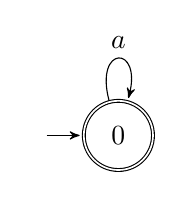
\begin{tikzpicture}[>=stealth', shorten >=1pt, auto,
    node distance=2cm,initial text={}]
    \node [state, initial, accepting]                         (A) {$0$};
    \path[->] (A) edge [loop above]             node {$a$} ();
  \end{tikzpicture}
  \caption{UFA}
  \label{fig:ufa}
\end{subfigure}
\begin{subfigure}{.5\textwidth}
  \centering
  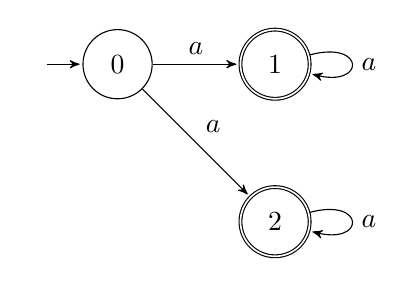
\begin{tikzpicture}[>=stealth', shorten >=1pt, auto,
    node distance=2cm,initial text={}]
    \node [state, initial]                           (A) {$0$};
    \node [state, accepting] [right of=A]            (B) {$1$};
    \node [state, accepting] [below of=B]            (C) {$2$};
    \path[->] (A) edge                          node {$a$} (B)
                  edge                          node {$a$} (C)
              (B) edge [loop right]             node {$a$} ()
              (C) edge [loop right]             node {$a$} ();
  \end{tikzpicture}
  \caption{FNFA}
  \label{fig:fnfa}
\end{subfigure}
\newline
\begin{subfigure}{.5\textwidth}
  \centering
  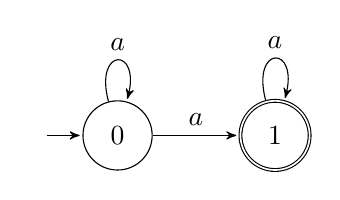
\begin{tikzpicture}[>=stealth', shorten >=1pt, auto,
    node distance=2cm,initial text={}]
    \node [state, initial]                           (A) {$0$};
    \node [state, accepting] [right of=A]            (B) {$1$};
    \path[->] (A) edge                          node {$a$} (B)
                  edge [loop above]             node {$a$} ()
              (B) edge [loop above]             node {$a$} ();
  \end{tikzpicture}
  \caption{PNFA}
  \label{fig:pnfa}
\end{subfigure}
\begin{subfigure}{.5\textwidth}
  \centering
  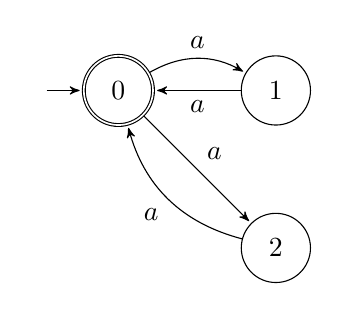
\begin{tikzpicture}[>=stealth', shorten >=1pt, auto,
    node distance=2cm,initial text={}]
    \node [state, initial, accepting]                (A) {$0$};
    \node [state] [right of=A]                       (B) {$1$};
    \node [state] [below of=B]                       (C) {$2$};
    \path[->] (A) edge [bend left]              node {$a$} (B)
                  edge                          node {$a$} (C)
              (B) edge                          node {$a$} (A)
              (C) edge [bend left]             node {$a$} (A);
  \end{tikzpicture}
  \caption{ENFA}
  \label{fig:enfa}
\end{subfigure}
\caption{Classes of Ambiguity}
\label{fig:automaton}
\end{figure}

\begin{definition}
An NFA is \emph{unambiguous} if, for each word $w$, there is at most one accepting path.
\end{definition}

Figure \ref{fig:ufa} shows an example of an NFA diagram that is \emph{unambiguous}. All accepted words have only one accepting path. Note that a DFA is always \emph{unambiguous} (but not all \emph{unambiguous} automata are DFA).

\begin{definition}
An NFA is \emph{finitely ambiguous} if there is a $k \in Z$ such that, for each word $w$, the number of paths that accepts $w$ is at most $k$.
\end{definition}

Figure \ref{fig:fnfa} shows an example of an NFA diagram that is \emph{finitely ambiguous}, where the accepted language is the language of the regular expression $aa^*$. The degree of ambiguity of the NFA is two.

\begin{figure}[ht]
\centering
\begin{tabular}{ccc}
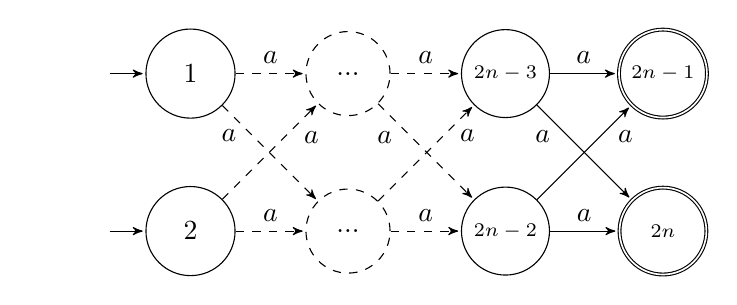
\begin{tikzpicture}[>=stealth', shorten >=1pt, auto,
  node distance=2cm,initial text={},text width=8mm,align=center]
  % \node [state, initial]                 (A) {$0$};
  % \node [state, initial]   [below of=A]  (B) {$1$};
  \node [state,initial]               (C) {$1$};
  \node [state,initial] [below of=C]  (D) {$2$};

  % \path[->] (A) edge                     node {$a$} (C)
  %               edge                     node {$a$} (D)
  %           (B) edge                     node {$a$} (C)
  %               edge                     node {$a$} (D);

  \node [state,dashed]   [right of=C]  (E) {$...$};
  \node [state,dashed]   [below of=E]  (F) {$...$};

  \node [state] [right of=E]                 (G) {\scriptsize $2n-3$};
  \node [state] [below of=G]                 (H) {\scriptsize $2n-2$};
  \node [state, accepting] [right of=G]      (I) {\scriptsize $2n-1$};
  \node [state, accepting] [right of=H]      (J) {\scriptsize $2n$};

  \path[->] (G) edge                         node {$a$} (I)
                edge                         node {$a$} (J)
            (H) edge                         node {$a$} (I)
                edge                         node {$a$} (J);

  \path[dashed,->] (C) edge     node {$a$} (E)
                       edge     node {$a$} (F)
                   (D) edge     node {$a$} (E)
                       edge     node {$a$} (F)
                   (E) edge     node {$a$} (G)
                       edge     node {$a$} (H)
                   (F) edge     node {$a$} (G)
                       edge     node {$a$} (H);
\end{tikzpicture} \\
\end{tabular}
\caption{Family of FNFA where the degree of ambiguity grows exponentially with the size of the automata}
\label{fig:FNFAexpo}
\end{figure}

\begin{lemma} \textbf{\cite{Seidl89}}
The degree of an FNFA of size $m$ is at most of the order $2^{O(m\times \log_2 m)}$.
\end{lemma}

In Figure \ref{fig:FNFAexpo} we can see an example of a family of FNFA diagram where the degree grows exponentially with the size of the automata.

An automaton of that family with $2n$ nodes, where $n>1$, will have (finite) degree of ambiguity of $2^{n/2}$ and will accept the language $a^{n-1}$.

\begin{definition}
An NFA is \emph{polynomially ambiguous} if there is a polynomial $p$ such that, for each word $w$, the number of paths that accepts $w$ is at most $p(|w|)$.
\end{definition}

Figure \ref{fig:pnfa} shows an example of a PNFA diagram  where the word $a^i, i \geq 1$, has $i$ accepting paths. An example of a polynomial that bounds the degree of ambiguity of the NFA mentioned is the identity polynomial $p(k) = k$.

\begin{definition}
An NFA is \emph{exponentially ambiguous} if, for each word $w$, the number of paths that accept $w$ is bounded by some exponential function on the size of $w$.
\end{definition}

An example of an ENFA diagram is shown in Figure \ref{fig:enfa} where the degree of the word $a^{2(i+1)}$ has $2^i$ accepting paths.

\section{Criteria for Ambiguity Classification}
To classify an automaton there are three criteria that can be checked. A criterion to check if an automaton is ambiguous, the Infinite Degree of Ambiguity (IDA) criterion to check if the degree is finite and the Exponential Degree of Ambiguity (EDA) criterion to check if an automaton has exponential ambiguity. There is an algorithm to check each criterion and they can be computed in polynomial time, therefore the classification of the ambiguity of an NFA can be decided in polynomial time.

In this section we present the criteria above and the newly written code to test the criteria of NFA's. The newly written auxiliary functions used in the code can be consulted in the appendix, except for the functions \emph{trim}, \emph{dup} and \emph{addTransition} that can be found in the documentation of FAdo \cite{BRODA201994}.

\subsection{Criterion for Exponential Degree of Ambiguity - EDA}
An NFA is ENFA if and only if it complies with the following EDA criterion \cite{Seidl89}.

EDA: there exists a state $q$ with at least two distinct cycles labeled by some $v \in \Sigma^*$.

The algorithm presented in Algorithm \ref{algorithm:eda} is based on the following lemma.

\begin{lemma} \textbf{\cite{AllauzenMR11}}
An NFA $M$ satisfies EDA if and only if there exists a strongly connected component of $M^2 = M \cap M$, obtained from the product, that contains two states of the form $(p,p)$ and $(q,q')$ with $p,q,q'$ states of $M$ and $q \neq q'$.
\end{lemma}

For an NFA $M$, the algorithm presented in Algorithm \ref{algorithm:eda}, is as follows. First, in lines 2-7, $M$ is trimmed and $M^2$ is computed.
Then we get the connected components of $M^2$ (line 9), and, for each one, we check if there are two states $(s_1,s_2),(s_1',s_2') \in M^2$ such that $s_1 = s_2 \land s_1' \neq s_2'$ (line 16).

%s1 < s2
\begin{lstlisting}[language=Python, caption = Algorithm to test EDA criterion, label={algorithm:eda}]
def testEDA(nfax):
    nfa = nfax.dup()
    nfa.trim()

    conj = myProduct(nfa,nfa)
    addFinals(conj, nfa, nfa)
    conj.trim()

    comp = stronglyConnectedComponents(conj)
    for l in comp:
        for s1 in l:
            for s2 in l:
                if s1==s2: continue
                (p1,p2) = literal_eval(conj.States[s1])
                (q1,q2) = literal_eval(conj.States[s2])
                if p1==p2 and q1!=q2:
                    return True
    return False
\end{lstlisting}

\subsection{Criterion for Infinite Degree of Ambiguity - IDA}
An NFA M is PNFA if and only if it complies with the following IDA criterion \cite{Seidl89} and not satisfies the EDA criterion.

IDA: There are distinct useful states $p,q \in Q$ such that for some word $v \in \Sigma^*$ $(p,v,p),(p,v,q),(q,v,q) \in \delta$.

The algorithm presented in Algorithm \ref{algorithm:ida} is based on the following lemma.

\begin{lemma} \textbf{\cite{AllauzenMR11}}
An NFA $M$ satisfies IDA if and only if there exist two different states $p$ and $q$ in $M$ with a path in $M^3=M \cap M \cap M$, obtained from the product, from state $(p,p,q)$ to state $(p,q,q)$.
\end{lemma}

For an NFA $M$, the algorithm presented in Algorithm \ref{algorithm:ida}, is as follows. First, in lines 2-11, $M$ is trimmed and $M^3$ is computed. Then, in lines 13-19, we add the transitions $((p,p,q),\#,(p,q,q))$ for all states $p,q$ of $M$ ($\#$ is a symbol that is not in the alphabet of $M$). %using function x and y
Finally, we get the connected components of $M^3$ (line 21), and, for each one, check if there is a transition by the new symbol $\#$ and by another in the original alphabet (lines 30-31).

\begin{lstlisting}[language=Python, caption = Algorithm to test IDA criterion, label={algorithm:ida}]
def testIDA(nfax):
    nfa = nfax.dup()
    nfa.trim()

    sz = len(nfa.States)

    conj = myProduct(nfa,nfa)
    addFinals(conj, nfa, nfa)

    conj2 = myProduct(conj,nfa)
    addFinals(conj2, conj, nfa)

    for p in xrange(0,sz):
        for q in xrange(0,sz):
            if p==q: continue
            a = (p*sz+p,q)
            b = (p*sz+q,q)
            conj2.addTransition(a[0]*sz+a[1],'#',b[0]*sz+b[1])
    conj2.trim()

    comp = stronglyConnectedComponents(conj2)
    for l in comp:
        tcard = False
        tother = False
        for i in l:
            if i not in conj2.delta: continue
            for symb in conj2.delta[i]:
                for t in conj2.delta[i][symb]:
                    if t in l:
                        if symb=='#': tcard = True
                        else: tother = True
                        if tcard and tother: return True

    return False
\end{lstlisting}


\subsection{Criterion for Having Ambiguity}
An NFA M is ambiguous if and only if in $M \times M$ there is a useful state that is not in the diagonal \cite{Sakarovitch}.

An automaton is FNFA if and only if it is ambiguous and not satisfies the IDA criterion. If it is not ambiguous then it is UFA.

% Finally the following algorithm tests whether an NFA $M$ is ambiguous by checking if it has some useful state that is not in the diagonal of $M^2$.
For an NFA $M$, the algorithm presented in Algorithm \ref{algorithm:amb}, is as follows. First, in lines 2-6, $M$ is trimmed and $M^2$ is computed. Then for each useful state of $M^2$ we test if it is in the diagonal (lines 10 and 11).

\begin{lstlisting}[language=Python, caption = Algorithm to test Ambiguity, label={algorithm:amb}]
def testAmbiguity(nfax):
    nfa = nfax.dup()
    nfa.trim()

    conj = myProduct(nfa,nfa)
    addFinals(conj, nfa, nfa)

    useful = conj.usefulStates()
    for i in useful:
        (x,y) = literal_eval(conj.States[i])
        if x != y:
            return True

    return False
\end{lstlisting}

\chapter{Results and their Discussion}
In this chapter we present the results of the experiment performed in order to evaluate the incidence of each class of ambiguity in NFA'a obtained from converting regular expressions. We considered two standard methods: Glushkov (also known as Position) \cite{glu61} and Antimirov (also known as Partial Derivatives or PD) \cite{Antimirov96}.
 % order to find the relation between the classes of ambiguity and the size of the automaton.

To perform the experiment $10000$ regular expressions were generated for each $n \in \{20$, $35$, $50$, $75$, $100\}$ and $k \in \{2$, $5$, $10\}$, where $n$ is the number of symbols in the expression excluding parentheses and $k$ is the size of the alphabet. Each regular expression was converted into two NFA's, one for each method of conversion.

% After the regular expressions were generated, for each one of them, we converted it to an NFA with the methods of \emph{Position} and \emph{Partial Derivatives} getting two NFA's .

The average size of the automata resulting from the conversion using the \emph{Position} method is $n/2$ and using the \emph{PD} method is $n/4$, where $n$ is the size of the regular expression \cite{BrodaMMR11}.

We classified the NFA's using the algorithms explained in the last chapter. The results are summarized in Figure \ref{fig:results}.

In the graphics of Figure \ref{fig:results} we can see that both methods have similar distributions. That was expected because it was proven that the \emph{PD} automaton is isomorphic to a quotient of \emph{Position} automaton \cite{IlieY03}.

The number of \emph{unambiguous automata} increases if the $k$ is large or when the $n$ is small.

In our results, PNFA is the class of ambiguity with the lowest presence.

Contrary to the \emph{unambiguous} automata, the number of \emph{exponential ambiguous} automata increases if the $n$ is large or when the $k$ is small.

\begin{figure}[]
  \hspace*{-2.3cm}
  \centering
  \begin{tabular}{cc}
    \includegraphics[width=0.6\columnwidth]{ufa} &   \includegraphics[width=0.6\columnwidth]{fnfa} \\
  (a) Unambiguous Automata & (b) Finitely Ambiguous Automata \\[6pt]
   \includegraphics[width=0.6\columnwidth]{pnfa} &   \includegraphics[width=0.6\columnwidth]{enfa} \\
  (c) Polinomially Ambiguous Automata & (d) Exponentially Ambiguous Automata \\[6pt]
  \end{tabular}
  \caption{Results}
  \label{fig:results}
\end{figure}

\chapter{Conclusion}

The ambiguity of an automaton is an important characteristic because if an NFA is \emph{unambiguous} many decision problems that are only solvable in exponential time become solvable in polynomial time (e.g equivalence of two automata \cite{StearnsH85}).

There are well-defined algorithms to classify the ambiguity class of an automaton that was implemented and used in this work. Besides the algorithms presented, there is also one to determine the smallest degree of the polynomial that bounds the ambiguity degree of a PNFA automaton \cite{Seidl89}.

However, there is no algorithm to determine the degree of an FNFA automaton except for finding the degree by some kind of brute force exploration of all words. It is also PSPACE-complete to decide if an FNFA automaton has degree $k, k>0$ \cite{ChanI83}.

Furthermore, the degree of ambiguity of an FNFA can be exponential in the size of the automaton \cite{Seidl89}. An example of a family of FNFA where the degree grows exponentially with the size of the automaton was shown in Figure \ref{fig:FNFAexpo}.

Finally, analyzing the results, we can see that most of the automata classified are \emph{exponentially ambiguous}. Which means that the most common class of ambiguity for automata (if it is the result from the conversion of a regular expression) is ENFA, and, since the ENFA is the one where the number of paths growths faster (exponentially), this leads to a more inefficient analysis of automata.

In order to get a more clear understanding of the ambiguity of automata, it is necessary more work to find an algorithm to compute the degree of ambiguity of an FNFA. An interesting line of work would be also to try to decrease and remove the ambiguity of an automaton.

\appendix
\chapter{Code for Auxiliary Functions}

\begin{lstlisting}[language=Python, caption = Auxiliary functions]
def addFinals(conj, nfa1, nfa2):
    """Adds finals states to nfa1 x nfa2"""
    sz = len(nfa2.States)
    for x in [(a, b) for a in nfa1.Final for b in nfa2.Final]:
        if str(x) in conj.States:
            conj.addFinal(x[0]*sz+x[1])

def myProduct(nfa1, nfa2):
    """Computes nfa1 x nfa2"""
    nfa = NFA()

    sz1 = len(nfa1.States)
    sz2 = len(nfa2.States)

    #state (i,j) is in index i*sz2+j
    for i in xrange(0,sz1):
        for j in xrange(0,sz2): nfa.addState(str((i,j)))
    for i in nfa1.Initial:
        for j in nfa2.Initial: nfa.addInitial(i*sz2+j)

    for s1 in nfa1.delta:
        for symb in nfa1.delta[s1]:
            for s2 in nfa2.delta:
                if symb not in nfa2.delta[s2]: continue
                states = [i*sz2+j for i in nfa1.delta[s1][symb] for j in nfa2.delta[s2][symb]]
                for state in states: nfa.addTransition(s1*sz2+s2,symb,state)
    return nfa

def stronglyConnectedComponents(nfa):
    """Computes the strongly connected components of nfa"""
    def dfs(graph, node, vis, list):
        stack = [node]
        while len(stack) > 0:
            n = stack.pop()
            if vis[n] == 2: continue
            if vis[n] == 1:
                list.append(n)
                vis[n] = 2
                continue

            vis[n] = 1
            stack.append(n)
            for child in graph[n]:
                if not vis[child]: stack.append(child)

    sz = len(nfa.States)
    graph  = [set() for i in xrange(0,sz)]
    graphT = [set() for i in xrange(0,sz)]

    for i in nfa.delta:
        for symb in nfa.delta[i]:
            for j in nfa.delta[i][symb]:
                graph[i].add(j)
                graphT[j].add(i)

    stack = []
    vis = [0 for i in xrange(0,sz)]
    for node in xrange(sz-1,-1,-1):
        if not vis[node]: dfs(graph, node, vis, stack)

    strongComp = []
    vis = [0 for i in xrange(sz-1,-1,-1)]
    while len(stack) > 0:
        node = stack.pop()
        if vis[node]: continue
        comp = []
        dfs(graphT, node, vis, comp)
        strongComp.append(comp)

    return strongComp
\end{lstlisting}

%\renewcommand{\bibname}{References}
\addcontentsline{toc}{chapter}{Bibliography}
\bibliographystyle{plain}
\bibliography{refs}

\end{document}
